\section{Concrete implementation}
\label{sec:concrete}

The operational semantics we have derived in the previous section
constitutes an abstract \emph{specification}: a semantics for which
non-interference is (obviously) true.  This specification can guide the
design of an information-flow calculus which would not be directly
derivable from our procedure, but is related to some such derivation.
For example, in our mini-ML language, the combined semantics requires
each thread to have a separate ML heap.  In an actual implementation, we
might like to only have a single heap, but disallowing the
passing of references between threads.  This restriction maintains a
correspondence between the abstract multiple heaps and the concrete
single heap.  As long as we don't add any extra transitions which directly
leak secret data, we might hope that non-interference follows
immediately.

However, when proving termination-\emph{sensitive} non-interference, we
cannot allow an arbitrary restrictions.  Consider a trivial state
machine as shown in Figure~\ref{fig:trivial-sm}, whose second projection
is classified secret.  With all three transitions, this language
fulfills termination-sensitive noninterference.  Furthermore, if the
dashed line is removed, the language continues to satisfy TSNI.
However, if any solid line is removed, however, the language fails TSNI.
Only \emph{some} transitions may be removed safely.

\begin{figure}
    States: $(x,y)$ for $x,y \in \{0,1\}$ \\
    Erasure function: $f(x,y) = (x,\bullet)$

    \begin{center}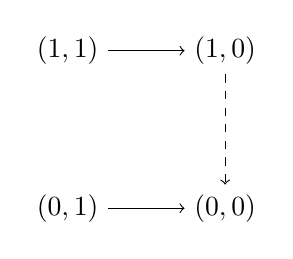
\begin{tikzpicture}[node distance=2cm, auto]
        \node (A) {$(1,1)$};
        \node (B) [right of=A] {$(1,0)$};
        \node (C) [below of=A] {$(0,1)$};
        \node (D) [right of=C] {$(0,0)$};
        \draw[->] (A) to node {} (B);
        \draw[->] (C) to node {} (D);
        \draw[->, dashed] (B) to node {} (D);
    \end{tikzpicture}\end{center}

    \label{fig:trivial-sm}
    \caption{A trivial state machine}
\end{figure}

In order to capture the condition with which transitions may be removed
safely, we require a novel, stronger variant of termination-sensitive
noninterference:

\begin{lemma}[Erased-transition/transition simulation (ETTS)]
    For any state |C|, if |erase l C ..-> delta|, then there exists a |C'| such that
    |erase l C' = delta| and |C .=> C'|.
\end{lemma}

Traditional TSNI is an easy corollary of this lemma.  \Red{Need to argue
this is provable!} Now we can state the result:

\begin{theorem}
    Suppose we have a abstract specification language $L$ with machine
    states $|C|$, evaluation relation $|.->|$, erasure function $|erasef l|$,
    and a proof that ETTS holds.

    Next, suppose we have a language $L'$ with machine states $|C'|$,
    evaluation relation $|.->|'$ and erasure function $|erasef l|'$.  We demand that this
    language be related to $L$ in the following way:

    \begin{itemize}
        \item There are functions $f : |C' -> C|$ and $f^{-1} : |C -> C'|$ which is functorial
            over $l$-equivalences: e.g. if $|C| \approx'_l |C'|$ then
            $f(|C|) \approx_l f(|C'|)$ and vice versa.
    \end{itemize}

    Then ETTS holds for language $L'$.
\end{theorem}

\begin{proof}
We need to show that for all choices of $|C1'|$, there exists a $|C2'|$ with
the desired properties.  We proceed by induction on the erased-transition.
There are two cases.  In the first case, there is a one-to-one correspondence
between reduction relations in 

Our proof proceeds along the same lines as a traditional TSNI proof,
we simply must show \Red{Lemma~1} holds for our language.  We proceed by induction
over reduction derivations in the first step.

We have $ts'_1 \approx_l ts'_2$ and would like to show $f(ts'_1) \approx_l f(ts'_2)$;
this can be seen by expanding the definition of
\end{proof}

To provide a sense of how these conditions work, we give an example
use of these theorem:

\begin{theorem}
    The language described in Figure X satisfies termination sensitive non-interference.
\end{theorem}

\begin{code}
\end{code}


\begin{figure}

\begin{mathpar}
\inferrule[I-stepT]
{|
conf tS (te) -> conf tS' te'
|}
{|
coconf iS tS (cconf id il (iniE (IT te)), ldots)
.->
iS ; tS' ; sched step (cconf id il (iniE (IT te')), ldots)
|}

\and
% This rule is not complete, needs the FV condition
\inferrule[C-fork]
{ 
|iS' = iS [ id' mapsto nil ]|\\
|it1 = cconf id il (iniE id')|\\
|itnew = cconf id' il (TI ie)|\\
|fresh (id')|
}
{|
coconf iS tS (lconf id il (iniE (fork ie)), ldots)
.->
iS'; tS; sched fork (it1, ldots, itnew)
|}
\end{mathpar}

\caption{ML with a single heap}
\label{fig:comb}
\end{figure}

This version
